%\section{Joan Nyria Hancox}\label{Joan_Nyria_Hancox}

\biohead{Joan Nyria Hancox}{Joan_Nyria_Hancox}{Late 1950s in Great Witley.\cite{FlickrNyria}}

%\begin{center}
%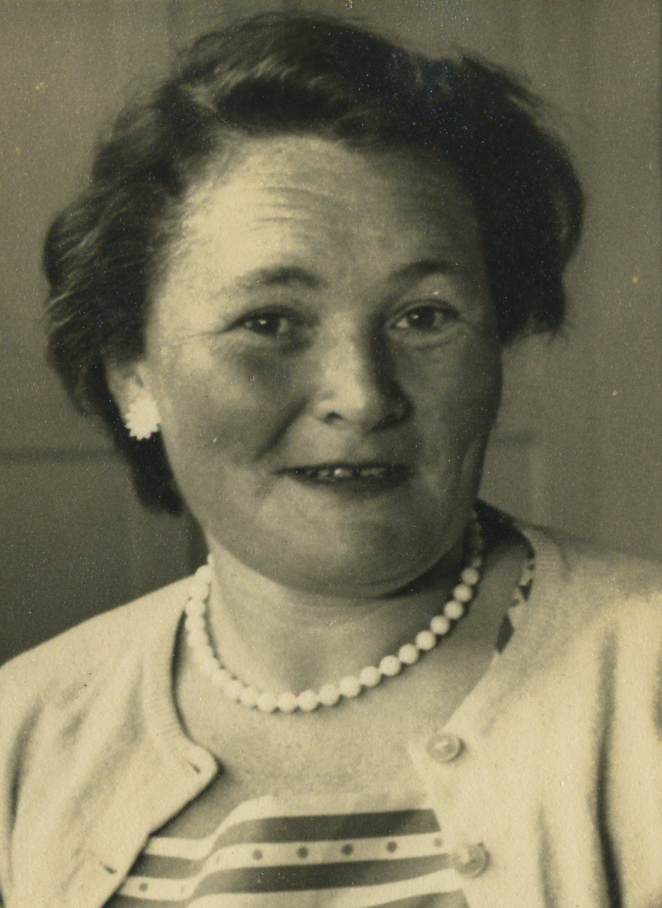
\includegraphics[width=0.8\linewidth]{photos/Joan_Nyria_Hancox} \\
%{\footnotesize Late 1950s in Great Witley.\cite{FlickrNyria}}
%\end{center}

\textbf{Nyria Denton-Barker (n\'{e}e Hancox)} (23 February 1918 -- 15 October 2004) was born in Bebington.\cite{BMDIndex_JoanNyriaHancox_birth}

Aged 6 (c.1925) she attended Howell's School Llandaff (in the Vale of Glamorgan, Wales).\cite{OralHistoryJDB2008}

In the mid-thirties she studied nursing at Guy's Hospital, where she was working as a Sister on the children's ward when, in 1938, she was evacuated out of London.

She died on 15 October 2004 in St Helens, Tasmania.
